\documentclass[11pt, oneside]{article}

% Packages
\usepackage{jmlr2e}
\usepackage{xcolor}
\usepackage[super]{nth}
\usepackage{mathtools, amsfonts}
\usepackage{graphicx}
\usepackage{subfig}

% Package config
% \sectionfont{\normalfont\sffamily\bfseries}
% \subsectionfont{\normalfont\sffamily\bfseries}
\hypersetup{colorlinks,
    linkcolor={red!50!black},
    citecolor={blue!50!black},
    urlcolor={blue!80!black}
}

% Notation and macros
%% Define bracket commands (normal, square and curly).
\newcommand{\brac} [1]  {\ensuremath{\left({#1}\right)}}
\newcommand{\sbrac}[1]  {\ensuremath{\left[{#1}\right]}}
\newcommand{\cbrac}[1]  {\ensuremath{\left\{{#1}\right\}}}
\newcommand{\abrac}[1]  {\ensuremath{\left\langle{#1}\right\rangle}}


%% Symbols

% General
\newcommand{\test}       {\ensuremath{^{*}}}
\newcommand{\testT}      {\ensuremath{^{*\top}\!}}
\newcommand{\ttest}      {\ensuremath{^{**}}}
\newcommand{\real}   [1] {\ensuremath{\mathbb{R}^{#1}}}
\newcommand{\natu}   [1] {\ensuremath{\mathbb{N}^{#1}}}
\newcommand{\ident}  [1] {\ensuremath{\mathbf{I}_{#1}}}

% Variables
\newcommand{\targs}     {\ensuremath{y}}
\newcommand{\targ}      {\ensuremath{\mathbf{y}}}
\newcommand{\targd}     {\ensuremath{\mathbf{y}\test}}
\newcommand{\targdT}    {\ensuremath{\mathbf{y}\testT}}
\newcommand{\ins}       {\ensuremath{\mathbf{X}}}
\newcommand{\inss}      {\ensuremath{\mathbf{x}}}
\newcommand{\locs}      {\ensuremath{\mathbf{z}}}
\newcommand{\minibatch}  {\ensuremath{\mathbf{B}}}
\newcommand{\feats}     {\ensuremath{\boldsymbol\Phi}}
\newcommand{\featfunc}  {\ensuremath{\boldsymbol\phi}}
\newcommand{\weights}   {\ensuremath{\mathbf{w}}}
\newcommand{\cov}       {\ensuremath{\boldsymbol{\Sigma}}}
\newcommand{\pocov}     {\ensuremath{\mathbf{C}}}
\newcommand{\lapcov}    {\ensuremath{\hat{\mathbf{C}}}}
\newcommand{\mcov}      {\ensuremath{\mathbf{S}}}
\newcommand{\jacob}[1]  {\ensuremath{\mathbf{J}_{#1}}}
\newcommand{\hess}[1]   {\ensuremath{\mathbf{H}_{#1}}}
\newcommand{\reg}       {\ensuremath{\lambda}}
\newcommand{\param}     {\ensuremath{\theta}}
\newcommand{\hyper}     {\ensuremath{\alpha}}
\newcommand{\lrate}     {\ensuremath{\eta}}

% Gaussian Process
\newcommand{\kernl}     {\ensuremath{k}}
\newcommand{\Kernl}     {\ensuremath{\mathbf{k}}}
\newcommand{\KERNL}     {\ensuremath{\mathbf{K}}}


%% Operations
\newcommand{\T}          {\ensuremath{^{\!\top}}}
\newcommand{\inv}        {\ensuremath{^{\text{-}1}}}
\newcommand{\deter}[1]   {\ensuremath{\left|{#1}\right|}}
\newcommand{\trace}[1]   {\ensuremath{\text{tr}\!\brac{#1}}}
\newcommand{\diag}[1]    {\ensuremath{\text{diag}\!\brac{#1}}}
\newcommand{\expec}[2]   {\ensuremath{\abrac{#2}_{\!{#1}}}}
\newcommand{\expece}[2]  {\ensuremath{\mathbb{E}_{#1}\!\sbrac{#2}}}
\newcommand{\evar} [2]   {\ensuremath{\mathbb{V}_{#1}\!\sbrac{#2}}}
\newcommand{\KL}[2]      {\ensuremath{\text{KL}\!\sbrac{{#1}\!\parallel\!{#2}}}}
\newcommand{\entropy}[1] {\ensuremath{\mathbb{H}\sbrac{#1}}}
\newcommand{\lnorm}[2]   {\ensuremath{\left\|{#2}\right\|_{{#1}}}}


%% Functions, PDFs etc
\newcommand{\func}  [2] {\ensuremath{f_{#2}\!\brac{{#1}}}}
\newcommand{\ofunc} [3] {\ensuremath{{#1}_{#3}\!\brac{{#2}}}}
\newcommand{\Prob}  [1] {\ensuremath{P\!\brac{#1}}}
\newcommand{\ProbC} [2] {\ensuremath{P\!\left({#1}\middle\vert{#2}\right)}}
\newcommand{\iProb}  [1] {\ensuremath{P\inv\!\brac{#1}}}
\newcommand{\iProbC} [2] {\ensuremath{P\inv\!\left({#1}\middle\vert{#2}\right)}}
\newcommand{\quant}  [1] {\ensuremath{Q\!\brac{#1}}}
\newcommand{\prob}  [1] {\ensuremath{p\!\brac{#1}}}
\newcommand{\probC} [2] {\ensuremath{p\!\left({#1}\middle\vert{#2}\right)}}
\newcommand{\qrob}  [1] {\ensuremath{q\!\brac{#1}}}
\newcommand{\qrobC} [2] {\ensuremath{q\!\left({#1}\middle\vert{#2}\right)}}
\newcommand{\gaus}  [1] {\ensuremath{\mathcal{N}\!\brac{#1}}}
\newcommand{\gausC} [2] {\ensuremath{\mathcal{N}\!\left({#1}\middle\vert{#2}\right)}}
\newcommand{\bern}  [1] {\ensuremath{\textrm{Bern}\!\brac{#1}}}
\newcommand{\bernC} [2] {\ensuremath{\textrm{Bern}\!\left({#1}\middle\vert{#2}\right)}}
\newcommand{\kfunc} [2] {\ensuremath{\kernl\!\brac{{#1}, {#2}}}}
\newcommand{\expon} [2] {\ensuremath{{#1}\!\times\!10^{#2}}}
\newcommand{\bigo}  [1] {\ensuremath{\mathcal{O}\!\brac{{#1}}}}
\newcommand{\elbo}      {\ensuremath{\mathcal{L}}}


%% Operators
\DeclareMathOperator*{\argmax}{\operatorname*{argmax}}
\DeclareMathOperator*{\argmin}{\operatorname*{argmin}}


% Preamble

% Heading arguments are
% {volume}{year}{pages}{submitted}{published}{author-full-names}
% \jmlrheading{}{}{}{}{}{}

% Short headings should be running head and authors last names
\ShortHeadings{\revrand{}~Technical Report}{Steinberg, Tiao, Reid, McCalman and
    O'Callaghan}
\firstpageno{1}

\title{\revrand{}: Technical Report}
\author{\name Daniel Steinberg \email daniel.steinberg@data61.csiro.au \\
        \name Louis Tiao \email louis.tiao@data61.csiro.au \\
        \name Alistair Reid \email alistair.reid@data61.csiro.au \\
        \name Lachlan McCalman \email lachlan.mccalman@data61.csiro.au \\
        \name Simon O'Callaghan \email simon.ocallaghan@data61.csiro.au \\
        \addr DATA61, CSIRO \\
        Sydney, Australia}

\date{}

\begin{document}

\maketitle
% \vspace{-0.5cm}
% \noindent\makebox[\linewidth]{\rule{\linewidth}{0.8pt}}
% \vspace{0.3cm}

\begin{abstract}
    This is a technical report on the \revrand{} software library. This
    library implements Bayesian linear models (Bayesian linear regression),
    generalized linear models and approximate Gaussian processes. These
    algorithms have been implemented such that they can be used for large-scale
    learning by using stochastic variational inference. All of the algorithms
    in \revrand{} use a unified feature composition framework that allows
    for easy concatenation and selective application of regression basis
    functions.
\end{abstract}

\tableofcontents

\section{Core Algorithms}

Recent developments in stochastic gradient optimisation have simplified the
application of machine learning to massive datasets, in particular, modern
stochastic optimisation algorithms are far more robust to initial learning rate
settings. Furthermore, Bayesian machine learning algorithms have a number of
well defined methods for learning model parameters and \emph{hyperparameters}
from training data, that do not involve cross validation. When used in
combination, stochastically optimized Bayesian machine learning algorithms
allow practitioners to learn probabilistic predictors from large data sets with
minimal tuning and retraining.

We make use of some of these recent developments in stochastic gradient methods
and stochastic variational inference in \revrand{} for supervisd regression
tasks. We outline the core algorithms implemented in \revrand{} in this section.

\subsection{Stochastic Gradients and Variational Objective Functions}
\label{sub:stochvar}

When a machine learning objective function factorises over data,
\begin{equation}
    \ffunc{\ins, \param}{} = \sum_{\inss \in \ins} \ffunc{\inss, \param}{},
\end{equation}
a regular gradient descent would perform the following iterations to minimise
the function w.r.t.\ the parameters $\param$,
\begin{equation}
    \param_k := \param_{k-1} - \lrate_k \sum_{\inss \in \ins}
    \nabla_{\param} \ffunc{\inss, \param}{}\!|_{\param = \param_{k-1}},
\end{equation}
where $\lrate_k$ is the learning rate (step size) at iteration $k$. Stochastic
gradients proposes the following update,
\begin{equation}
    \param_k := \param_{k-1} - \lrate_k \sum_{\inss \in \minibatch}
    \nabla_{\param} \ffunc{\inss, \param}{}\!|_{\param = \param_{k-1}},
    \label{eq:sg}
\end{equation}
where $\minibatch \subset \ins$ is a mini-batch of the original dataset, where
$|\minibatch| \ll |\ins|$.
Frequently objective functions to not entirely decompose over the data, i.e.,
\begin{equation}
    \ffunc{\ins, \param}{} = \sum_{\inss \in \ins} \ffunc{\inss, \param}{}
    + \func{g}{\param}{}.
    \label{eq:objwconst}
\end{equation}
However, it is trivial to make these objectives work in a stochastic gradient
setting. Let $M = |\minibatch|$ and $N = |\ins|$, then we divide the
contribution of the constant term amongst the mini-batches in stochastic 
gradients,
\begin{equation}
    \param_k := \param_{k-1} - \lrate_k \sum_{\inss \in \minibatch}
    \nabla_{\param} \ffunc{\inss, \param}{}\!|_{\param = \param_{k-1}}
    - \frac{M}{N} \lrate_k \nabla_{\param} 
    \func{g}{\param}{}\!|_{\param = \param_{k-1}}.
    \label{eq:wsg}
\end{equation} 
or, equivalently, boost the contribution of the mini-batch,
\begin{equation}
    \param_k := \param_{k-1} - \frac{N}{M} \lrate_k \sum_{\inss \in \minibatch}
    \nabla_{\param} \ffunc{\inss, \param}{}\!|_{\param = \param_{k-1}}
    - \lrate_k \nabla_{\param} 
    \func{g}{\param}{}\!|_{\param = \param_{k-1}}.
    \label{eq:wsg2}
\end{equation} 
This is particularly relevant for variational inference where the evidence
lower bound objective has a component independent of the data. For example, 
lets consider the model,
\begin{align}
    \text{Likelihood:} \quad &\prod^N_{n=1} \probC{\targs_n}{\param}, \\
    \text{prior:} \quad &\probC{\param}{\hyper},
\end{align}
where we want to learn the values of the hyper-parameters, $\hyper$. Minimising
negative log-marginal likelihood is a good objective in this instance, since we
don't care about the value(s) of $\param$,
\begin{equation}
    \argmin_\hyper - \log \int \prod^N_{n=1} \probC{\targs_n}{\param}
    \probC{\param}{\hyper} d \param.
    \label{eq:lml}
\end{equation}
There are two problems with this objective however, (1) it may not factor over
data and (2) the integral may be intractable, for instance, if the prior and
likelihood are not conjugate. In variational inference we use Jensen's
inequality to lower-bound log-marginal likelihood with a tractable objective
function called the evidence lower bound (ELBO),
\begin{align}
    \log \probC{\targ}{\hyper} =& \log \int 
        \prod^N_{n=1} \probC{\targs_n}{\param} 
        \probC{\param}{\hyper} d \param \nonumber \\
        =& \log \int 
        \frac{\prod_n \probC{\targs_n}{\param} \probC{\param}{\hyper}}
        {\qrob{\param}} \qrob{\param} d \param \nonumber \\
        \geq& \int \qrob{\param} \log \sbrac{%
            \frac{\prod_n \probC{\targs_n}{\param} 
            \probC{\param}{\hyper}}{\qrob{\param}}}
        d \param
\end{align}
where $\qrob{\param}$ is an approximation of $\probC{\param}{\hyper}$ that 
makes inference easier. This can be re-written as,
\begin{equation}
    \elbo = \sum^N_{n=1} \expec{q}{\log\probC{\targs_n}{\param}} -
    \KL{\qrob{\param}}{\probC{\param}{\hyper}},
    \label{eq:elbo}
\end{equation}
which takes the form of Equation~\eqref{eq:objwconst}, and so if we use
stochastic gradients optimisation we can weight the Kullback-Leibler term like
the constant term, $\func{g}{\cdot}{}$, from Equation~\eqref{eq:wsg}, or boost
the expected log likelihood term like in Equation~\eqref{eq:wsg2}.


\subsection{Bayesian Linear Regression -- \texttt{StandardLinearModel}}

The first machine learning algorithm in \revrand{} is a simple Bayesian linear
regressor of the following form,
\begin{align}
    \text{Likelihood:} \quad &\prod^N_{n=1} 
    \gausC{\targs_n}{\feats_n\T\weights, \var}, \label{eq:slm_like}\\
    \text{prior:} \quad &\gausC{\weights}{\mathbf{0}, \Reg},
    \label{eq:slm_prior}
\end{align}
where $\feats_n := \func{\featsym}{\inss_n, \param}{}$ is a feature, or basis,
function that maps $\featsym : \real{d} \to \real{D}$, and $\Reg \in
\real{D\times D}$ is a diagonal matrix (i.e.~it could be $\reg\ident{D}$) that
has the effect of regularising the magnitude of the weights. This is the same
algorithm described in~\citet[Chapter 2]{Rasmussen2006}. We then:
\begin{itemize}
    \item Optimise $\var, \Reg$ and $\param$ w.r.t.\ log-marginal likelihood,
        \begin{equation}
            \log \probC{\targ}{\var, \Reg, \param} =
            \log \gausC{\targ}{\mathbf{0}, \var\ident{N} + \feat\T\Reg\feat},
        \end{equation}
        where $\feat \in \real{N \times D}$ is the concatenation of all the
        features, $\feats_n$. Note this results in the covariance of the
        log-marginal likelihood being $N \times N$, though we can use the
        Woodbury identity to simplify the corresponding matrix inversion.
    \item Solve analytically for the posterior over weights, $\weights | \targ
        \sim \gaus{\pomean, \pocov}$ given the above hyperparameters, where,
        \begin{align*}
            \pocov &= \sbrac{\Reg\inv + \frac{1}{\var}
                \feat\T \feat}\inv, \\
            \pomean &= \frac{1}{\var} \pocov \feat\T \targ.
        \end{align*}
    \item Use the predictive distribution
        \begin{align}
            \probC{\targs\test}{\targ, \ins, \inss\test} &= \int
            \gausC{\targs\test}{\feats\testT\weights, \var}
            \gausC{\weights}{\pomean, \pocov} d\weights, \nonumber \\
            &= \gausC{\targs\test}{\feats\testT \pomean,
                \var + \feats\testT \pocov \feats\test}
        \end{align}
        for query inputs, $\inss\test$. This gives us the useful expectations,
        \begin{align}
            \expece{}{\targs\test} &= \feats\testT\pomean, \\
            \evar{}{\targs\test} &= \var + \feats\testT\pocov\feats\testT.
        \end{align}
\end{itemize}

It is actually easier to use the ELBO form with stochastic gradients for
learning the parameters of this algorithm, rather than log-marginal likelihood
recast using the Woodbury identity.  This is because it is plainly in the same
form as Equation \eqref{eq:objwconst}, though it would give the same result as
log-marginal likelihood because the ``approximate'' posterior is the same form
as the true posterior, i.e.\ $\qrob{\weights} = \gausC{\weights}{\pomean,
    \pocov}$. The ELBO for this model is,
\begin{equation}
    \elbo = \sum^N_{n=1} 
    \expec{q}{\log\gausC{\targs_n}{\feats_n\T\weights, \var}}
    - \KL{\gausC{\weights}{\pomean, \pocov}}
        {\gausC{\weights}{\mathbf{0}, \Reg}}.
    \label{eq:slmobj}
\end{equation}
More specifically,
\begin{align*}
    \expec{q}{\log\gausC{\targs_n}{\feats_n\T\weights, \var}} &=
    \log \gausC{\targs_n}{\feats_n\T\pomean, \var}
    - \frac{1}{2 \var} \trace{\feats_n\T\feats_n\pocov}, \\
    \KL{\gausC{\weights}{\pomean, \pocov}}
        {\gausC{\weights}{\mathbf{0}, \Reg}} &=
        \frac{1}{2} \sbrac{\trace{\Reg\inv\pocov} + \pomean\T\Reg\inv\pomean 
        -  \log\deter{\pocov} + \log\deter{\Reg} - D}
\end{align*}
We have not implemented a stochastic gradient version of this algorithm since
it still requires a matrix solve of a $D \times D$ matrix, and so is \bigo{D^3}
in complexity, per iteration. This is true even if we optimise the posterior
covariance directly (or a triangular parameterisation). The GLM presented in
the next section circumvents this issue, and is more suited to really large $N$
and $D$ problems.


\subsection{Bayesian Generalized Linear Models --
    \texttt{GeneralizedLinearModel}}

The algorithm of primary interest in \revrand{} is the Bayesian generalized
linear model. The general form of the model implemented by this algorithm is,
\begin{align}
    \text{Likelihood:} \quad &\prod^N_{n=1} 
        \probC{\targs_n}{\activ{\feats_n\T\weights}, \lparam}, 
        \label{eq:glm_like} \\
    \text{prior:} \quad &\gausC{\weights}{\mathbf{0}, \Reg},
        \label{eq:glm_prior}
\end{align}
for an arbitrary univariate likelihood, $\prob{\cdot}$, with an appropriate
transformation (inverse link) function, $\activ{\cdot}$, and parameter(s),
$\lparam$. 

Naturally, both calculating the exact posterior over the weights,
$\probC{\weights}{\targ, \ins}$, and the log-marginal likelihood,
$\prob{\targ}$, for hyperparameter learning are intractable since we may have a
non-conjugate relationship between the likelihood and prior. Therefore we must
resort to approximating the true posterior and the log-marginal likelihood.

Firstly, we approximate the true posterior over weights with a mixture of $K$
diagonal Gaussians,
\begin{align}
    \probC{\weights}{\targ, \ins} &\approx \qrob{\weights}, \nonumber \\
    &= \frac{1}{K} \sum^K_{k=1} \gausC{\weights}{\pomean_k, \dpocov_k},
\end{align}
where $\dpocov_k = \diag{[\dpocovs_{k,1}, \ldots, \dpocovs_{k, D}]\T}$, which
is inspired from similar approximations made in \citet{gershman2012,
    nguyen2014automated}. This is a very flexible form for the approximate
posterior, and has the nice property that our algorithm no longer has a
\bigo{D^3} cost associated with the number of features.

Then we approximate the log marginal likelihood using auto-encoding variational
Bayes \citep{kingma2014auto}. The exact lower bound on log marginal likelihood
is,
\begin{equation}
    \elbo = \sum^N_{n=1} 
    \expec{q}{\log\probC{\targs_n}{\activ{\feats_n\T\weights}, \lparam}}
    - \KL{\textstyle\frac{1}{K}\textstyle\sum_{k}
            \gausC{\weights}{\pomean_k, \dpocov_k}}
        {\gausC{\weights}{\mathbf{0}, \Reg}}.
    \label{eq:glmobj}
\end{equation}
This can be expanded,
\begin{multline}
    \elbo = \frac{1}{K} \sum^K_{k=1} \sum^N_{n=1} 
    \expec{q_k}{\log\probC{\targs_n}
        {\activ{\feats_n\T\weights}, \lparam}}
    + \frac{1}{K} \sum^K_{k=1}
        \expec{q_k}{\log\gausC{\weights}{\mathbf{0}, \Reg}} \\
    + \entropy{\textstyle\frac{1}{K}\textstyle\sum_{k}
            \gausC{\weights}{\pomean_k, \dpocov_k}},
    \label{eq:glmobj_exp}
\end{multline}
but unfortunately there are two intractable integrals here, the expected log
likelihood, and the entropy of the Gaussian mixture. We can use the lower bound
on the entropy term also used in \citet{gershman2012, nguyen2014automated},
\begin{equation}
    \entropy{\textstyle\frac{1}{K}\textstyle\sum_{k}
        \gausC{\weights}{\pomean_k, \dpocov_k}} \geq
    - \frac{1}{K} \sum_{k=1}^K \log \sum_{j=1}^K \frac{1}{K}
    \gausC{\pomean_k}{\pomean_j, \dpocov_k + \dpocov_j}.
\end{equation}
We can then use the reparameterisation trick in auto-encoding variational Bayes
\citep{kingma2014auto} to sample the expected log likelihood,
\begin{equation}
    \sum^N_{n=1} 
    \expec{q_k}{\log\probC{\targs_n}
        {\activ{\feats_n\T\weights}, \lparam}} \approx
    \frac{1}{L} \sum^{L}_{l=1} \sum^N_{n=1} \log\probC{\targs_n}
    {\activ{\feats_n\T\hat{\weights}_k^{\brac{l}}}, \lparam}
\end{equation}
where,
\begin{equation}
    \hat{\weights}_k^{\brac{l}} =
    \func{f}{\pomean_k, \dpocov_k, \resamp^{(l)}}{k} =
    \pomean_k + \sqrt{\dpocov_k} \odot \resamp^{(l)},
    \qquad \resamp^{(l)} \sim \gaus{\mathbf{0}, \ident{D}}.
\end{equation}
Here $\odot$ is the element-wise product. We can also use this trick to compute
approximate derivatives, $\frac{\partial}{\partial \alpha}
\expec{q(\alpha)}{\log \probC{\targs}{\alpha}} \approx \frac{1}{L} \sum^L_{l=1}
\frac{\partial}{\partial\alpha} \log \probC{\targs}{\func{f}{\alpha,
        \resamp^{(l)}}{}}$, which simplifies the implementation greatly! The
final auto-encoding variational Bayes objective for our GLM is,
\begin{multline}
    \elbo \approx \frac{1}{K} \sum^K_{k=1} \Bigg[
    \frac{1}{L} \sum^L_{l=1} \sum^N_{n=1} 
    \log\probC{\targs_n}
    {\activ{\feats_n\T \hat{\weights}_k^{\brac{l}}}, \lparam}
    + \log\gausC{\pomean_k}{\mathbf{0}, \Reg}
    - \frac{1}{2} \trace{\Reg\inv\dpocov_k} \\
    - \log \sum_{j=1}^K \frac{1}{K}
    \gausC{\pomean_k}{\pomean_j, \dpocov_k + \dpocov_j}
    \Bigg].
    \label{eq:glmobj_exp}
\end{multline}
We can straight forwardly use this objective within a stochastic gradients
setting using with the tactic in Equations \eqref{eq:wsg} or \eqref{eq:wsg2}.

The most simple and accurate method for approximating the predictive
distribution, $\probC{\targs\test}{\targ, \ins, \inss\test}$ is to Monte-Carlo
sample the integral,
\begin{equation}
    \probC{\targs\test}{\targ, \ins, \inss\test} \approx
    \int \probC{\targ}{\activ{\feats\testT\weights}, \lparam}
    \frac{1}{K} \sum^K_{k=1} \gausC{\weights}{\pomean_k, \dpocov_k} d \weights.
    \label{eq:glppred}
\end{equation}
However, this integral is not particularly useful unless we wish to evaluate
known $\targ\test$ under the model. For prediction, it is more useful to
compute (using Monte-Carlo integration) the predictive expectation, 
\begin{align}
    \expece{}{\targs\test} \approx&
    \int \frac{1}{K} \sum^K_{k=1} \gausC{\weights}{\pomean_k, \dpocov_k}
    \int \targs\test \probC{\targs\test}{\activ{\feats\testT\weights}, \lparam}
    d \targs\test d \weights
    \nonumber\\
    =& \int \expece{}{\probC{\targs\test}
        {\activ{\feats\testT\weights}, \lparam}}
    \frac{1}{K} \sum^K_{k=1} \gausC{\weights}{\pomean_k, \dpocov_k}
    d \weights.
    \label{eq:glmexpec}
\end{align}
Often we find $\expece{}{\probC{\targs\test}{\activ{\feats\testT\weights},
        \lparam}} = \activ{\feats\testT\weights}$, however this is only true
with with right choice and usage of the activation function. Furthermore, it is
useful to compute quantiles of the predictive density in order to ascertain the
predictive uncertainty. We start by sampling the predictive cumulative density
function, $\Prob{\cdot}$,
\begin{align}
    &\ProbC{\targs\test \leq \cdfAlph}{\targ, \ins, \inss\test} \nonumber\\ 
    &\qquad\approx \int 
    \frac{1}{K} \sum^K_{k=1} \gausC{\weights}{\pomean_k, \dpocov_k}
    \int^{\cdfAlph}_{-\infty} 
    \probC{\targs\test}{\activ{\feats\testT\weights}, \lparam}
    d \targs\test d \weights \nonumber\\
    &\qquad= \int
    \ProbC{\targs\test \leq \cdfAlph}{\activ{\feats\testT\weights}, \lparam}
    \frac{1}{K} \sum^K_{k=1} \gausC{\weights}{\pomean_k, \dpocov_k}
    d \weights.
    \label{eq:lapexpec}
\end{align}
Once we have obtained sufficient samples from the (mixture) posterior we can
obtain quantiles, $\cdfAlph$, for some chosen level of probability, $p$, using
root finding techniques. Specifically, we use root finding techniques to solve
the following for $\cdfAlph$,
\begin{equation}
    \ProbC{\targs\test \leq \cdfAlph}{\targ, \ins, \inss\test} - p = 0.
\end{equation}

\subsection{Large Scale Gaussian Process Approximation}

In \revrand{} we approximate Gaussian Processes \citep{Rasmussen2006} with
our standard and generalized linear models by using random feature functions
such as those of \citeauthor{rahimi2007} \citeyearpar{rahimi2007,rahimi2008}
and \cite{le2013fastfood}. They use Bochner's theorem regarding the
relationship between a kernel and the Fourier transform of a non-negative
measure (e.g.~a probability measure) that establishes the duality of the
covariance function of a stationary process and its spectral density,
\begin{align}
	\kernl(\tfourier) &= \int \specfourier(\ffourier) 
    e^{i \ffourier\T  \tfourier} d \ffourier,  \\
	\specfourier(\ffourier) &= \int \kernl(\tfourier) 
    e^{- i \ffourier\T \tfourier}  d \tfourier.
	\label{eq:fourier}
\end{align}
where $\kernl(\cdot)$ is a kernel function, and $\specfourier(\cdot)$ its
spectral density. \citeauthor{rahimi2007}'s  main insight
\citeyearpar{rahimi2007} is that we can approximate the kernel by constructing
`suitable' random features and Monte Carlo averaging over samples from
$\specfourier(\ffourier)$ for \emph{shift invariant} kernels,
\begin{equation}
    \kernl(\inss - \inssprime) = \kernl(\tfourier) 
    \approx \frac{1}{D} \sum_{i=1}^{D} \singlefeatfunc{\inss}{i}\T\!
	\singlefeatfunc{\inssprime}{i},
	\label{eq:mcapprox}
\end{equation}
$\singlefeatfunc{\inss}{i}$ corresponds to the $i$th sample from the feature
map. An example of a radial basis kernel feature vector construction using the 
above approximation is,
\begin{align}
	\nonumber
    \sbrac{\singlefeatfunc{\inss}{i}, \singlefeatfunc{\inss}{D+i}}&= 
    \frac{1}{\sqrt{D}} \sbrac{\cos(\ffourier_i^T \inss), 
    \sin(\ffourier_i^T \inss)}, \qquad \\
    \text{with}~\ffourier_i & \sim 
    \gausC{\ffourier_i}{\mathbf{0}, \lenscale\inv \ident{d}},
\end{align}
for $i=1, \ldots, D$,  which in fact is a mapping into a $2 D$-dimensional
feature space. See Table~\ref{tab:randommappings} for some of the random kernel
approximations we use in \revrand{}.

\begin{table}[htb]

    \centering

    \caption{Kernels and the corresponding Fourier weight ($\ffourier_i$)
        sampling distributions for the \citet{rahimi2007}-style random bases in
        \revrand{}. Here GAL refers to a multivariate Laplace
        distribution~\cite{kozubowski2013multivariate}.}

    \begin{tabular}{r|c c}
        \textbf{Kernel} & $\kernl\!\brac{\inss - \inssprime}$
        & $\specfourier(\ffourier)$ \\
        \hline
        RBF &
        $\exp\brac{-\frac{\lnorm{}{\inss - \inssprime}^2}{2\lenscale^2}}$ &
            $\ffourier_i \sim \gaus{\mathbf{0}, \lenscale\inv\ident{d}}$, \\
        Laplace & $\exp\brac{-\frac{\lnorm{}{\inss-\inssprime}}{\lenscale}}$ &
            $\ffourier_i \sim \prod_d \text{Cauchy}\!\brac{\lenscale\inv}$ \\
        Cauchy &
            $\frac{1}{1+\brac{\lnorm{}{\inss-\inssprime}/\lenscale}^2}$ & 
            $\ffourier_i \sim \text{GAL}\brac{1, \mathbf{0},
                \lenscale\inv\ident{d}}$ \\
        Matern $3/2$ & 
            $\brac{1 + \frac{\sqrt{3}\lnorm{}{\inss-\inssprime}}{\lenscale}}
            \exp\brac{-\frac{\sqrt{3}\lnorm{}{\inss-\inssprime}}{\lenscale}}$ & 
            $\ffourier_i \sim 
            \text{t}_{\nu=3}\!\brac{\mathbf{0}, \lenscale\inv\ident{d}}$ \\
        Matern $5/2$ &
            $\brac{1 + \frac{\sqrt{5}\lnorm{}{\inss-\inssprime}}{\lenscale} + 
                \frac{5\lnorm{}{\inss - \inssprime}^2}{3\lenscale^2}}
            \exp\brac{-\frac{\sqrt{5}\lnorm{}{\inss-\inssprime}}{\lenscale}}$ & 
            $\ffourier_i \sim 
            \text{t}_{\nu=5}\!\brac{\mathbf{0}, \lenscale\inv\ident{d}}$ \\
        \hline
    \end{tabular}

    \label{tab:randommappings}

\end{table}

All of the kernel functions in Table \ref{tab:randommappings} have length scale
hyperparameters, and in \revrand{} these can be isotropic or anisotropic length
scales that are learned alongside the other hyperparameters. We have also
implemented a few other variants of these random basis functions, namely the
Fastfood \citep{le2013fastfood} and A la Carte \citep{yang2014} basis functions
that improve scalability and representational flexibility respectively. In
Figure \ref{fig:kerns} we compare the basis approximations with their
corresponding kernels. We refer the reader to our demo notebooks for further
discussion and experiments comparing these approximate basis functions and the
kernels they approximate.

\begin{figure}[htb]
    \centering
    \subfloat[][RBF]{
        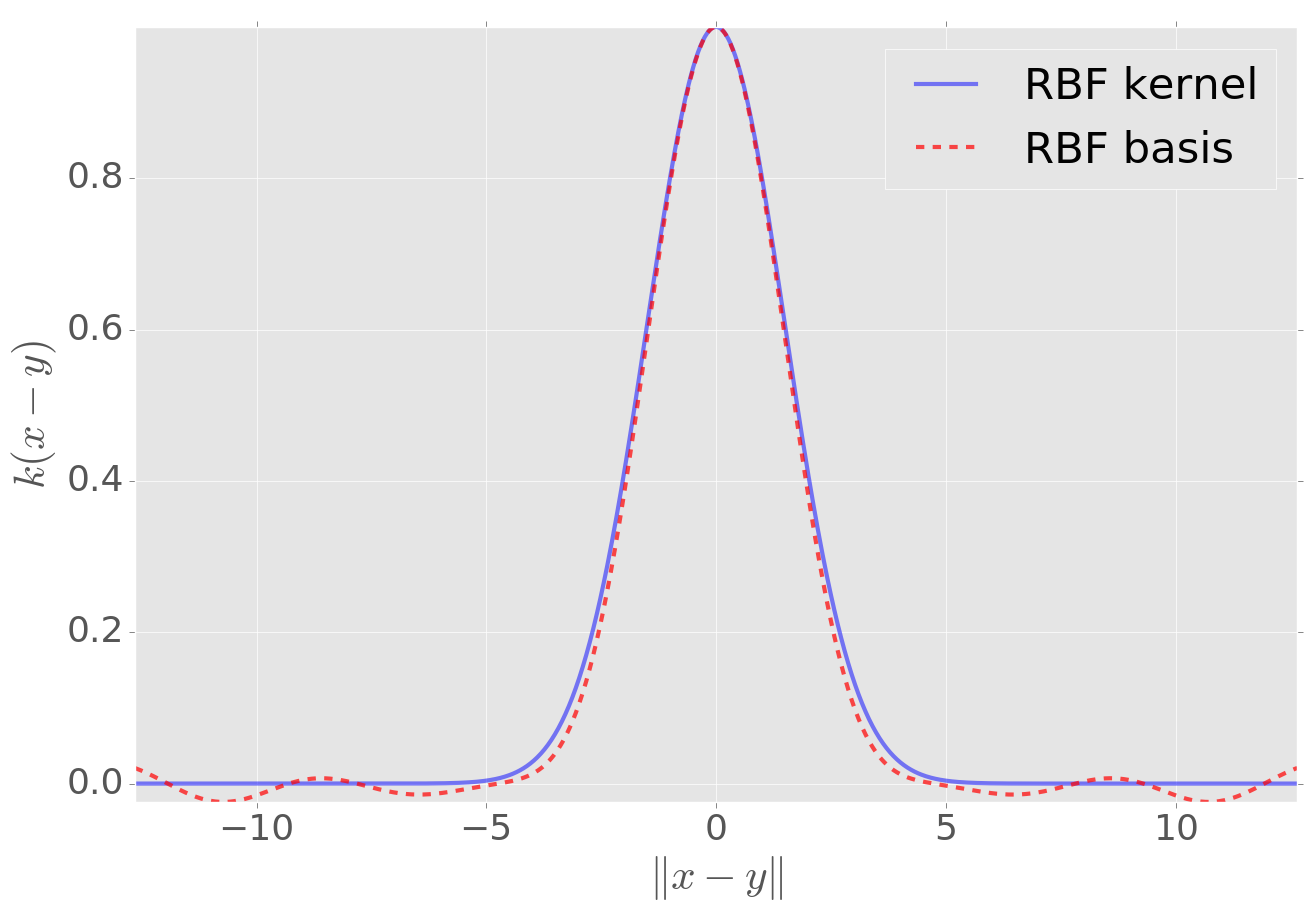
\includegraphics[width=0.47\linewidth]{figs/rbf.png}
        \label{fig:rbf}
    }
    \subfloat[][RBF Fastfood]{
        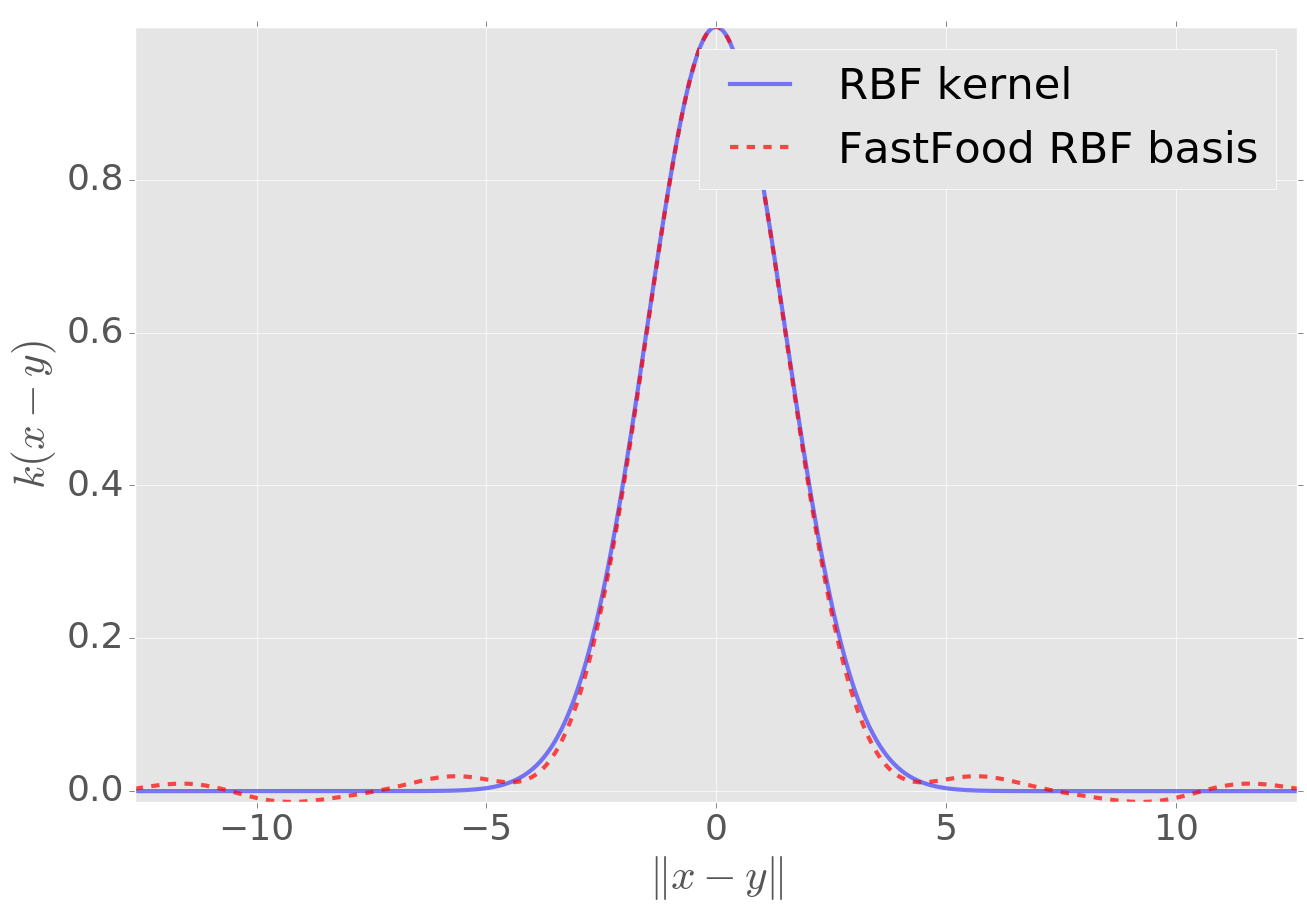
\includegraphics[width=0.47\linewidth]{figs/rbfFF.png}
        \label{fig:rbfFF}
    }\\
    \subfloat[][Laplace]{
        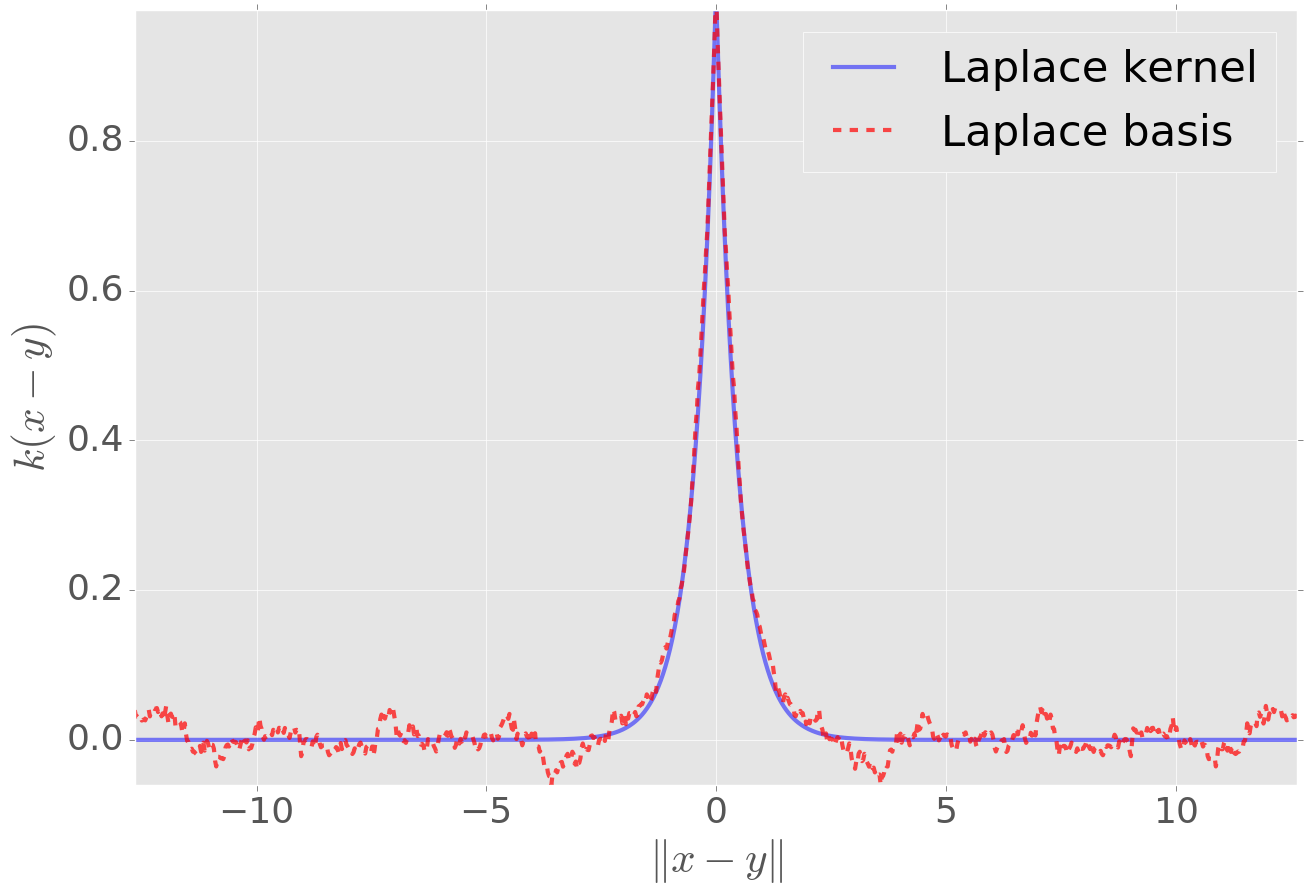
\includegraphics[width=0.47\linewidth]{figs/laplace.png}
        \label{fig:laplace}
    }
    \subfloat[][Cauchy]{
        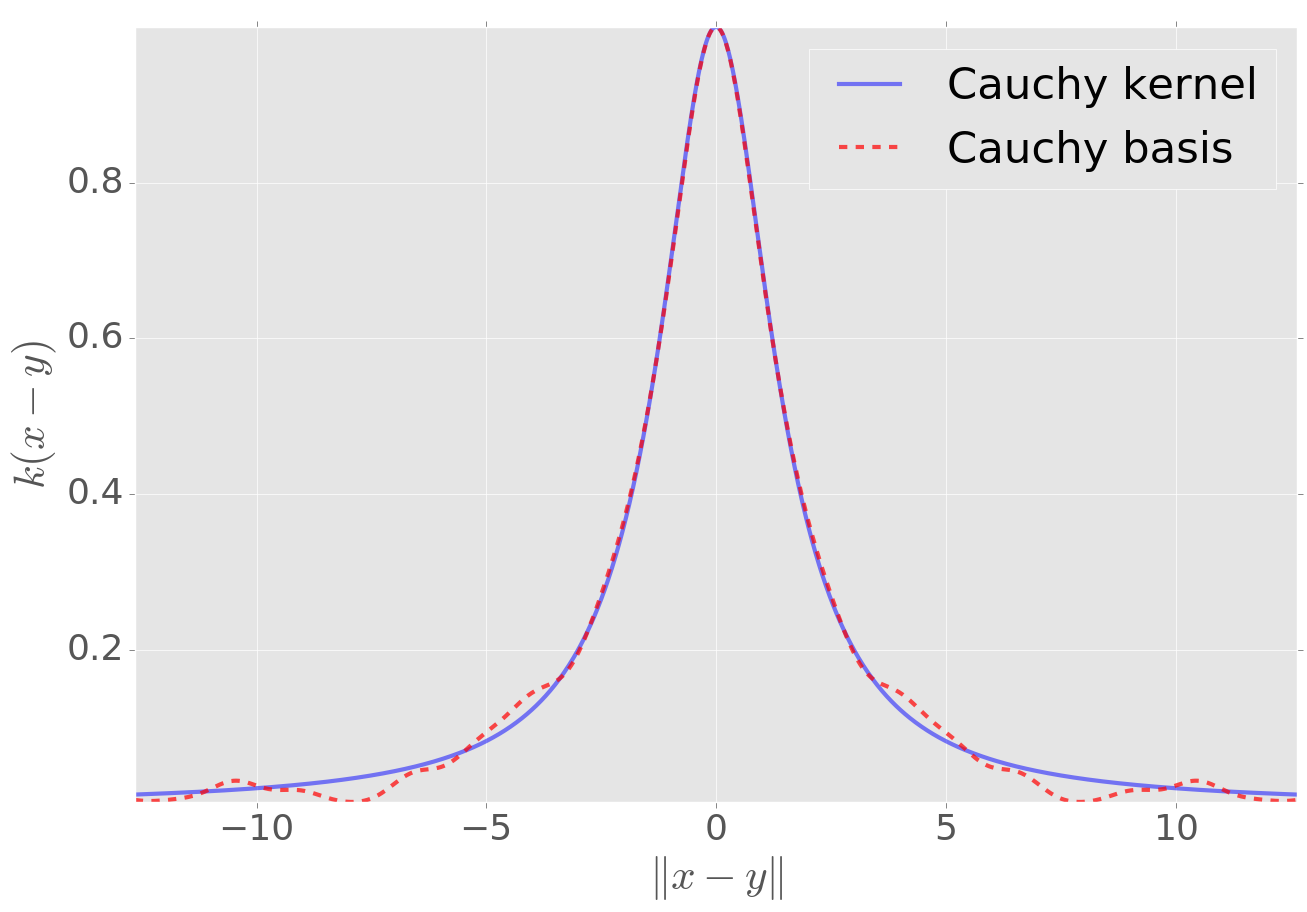
\includegraphics[width=0.47\linewidth]{figs/cauchy.png}
        \label{fig:cauchy}
    }\\
    \subfloat[][Matern 3/2]{
        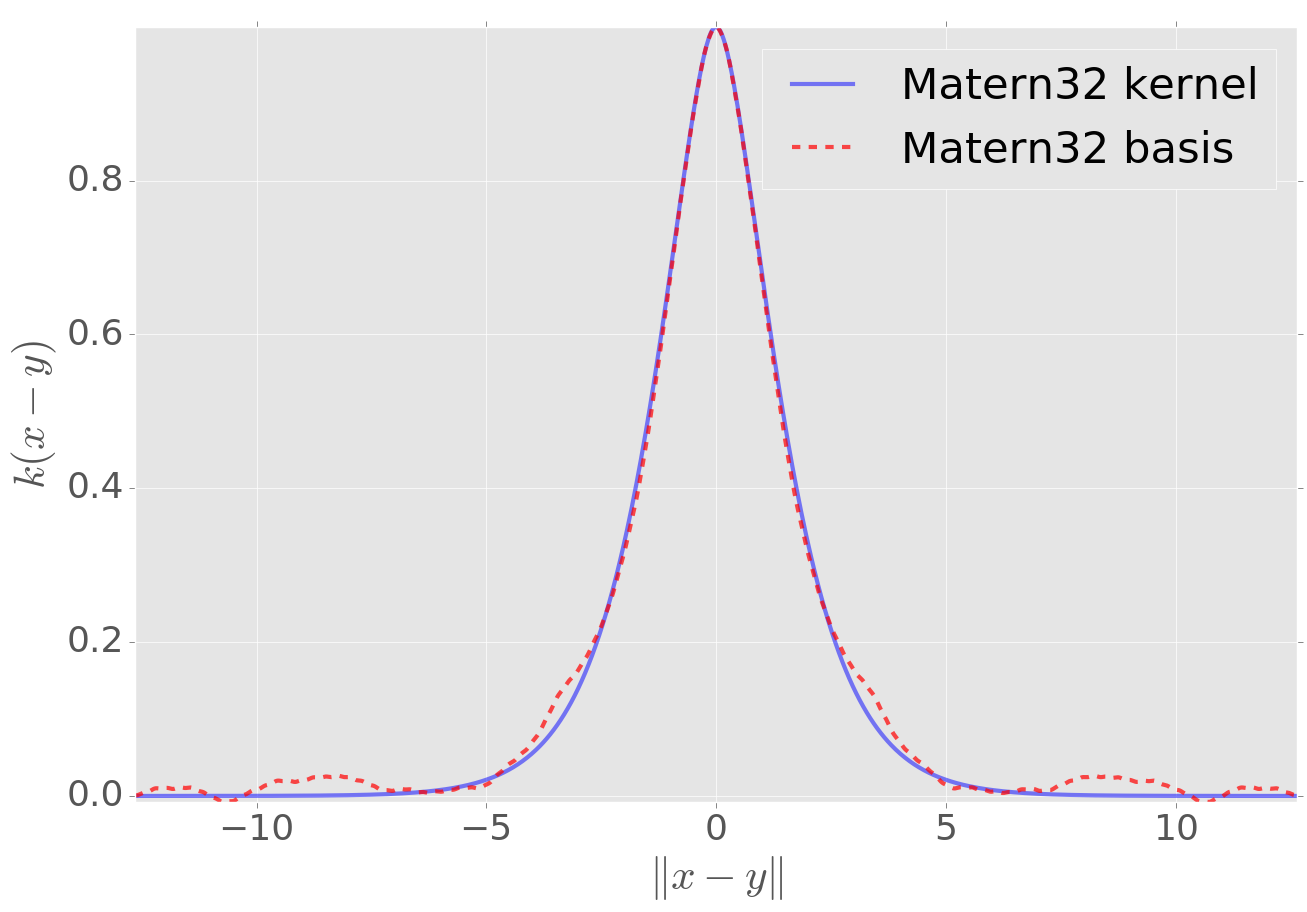
\includegraphics[width=0.47\linewidth]{figs/matern32.png}
        \label{fig:matern32}
    }
    \subfloat[][Matern 5/2]{
        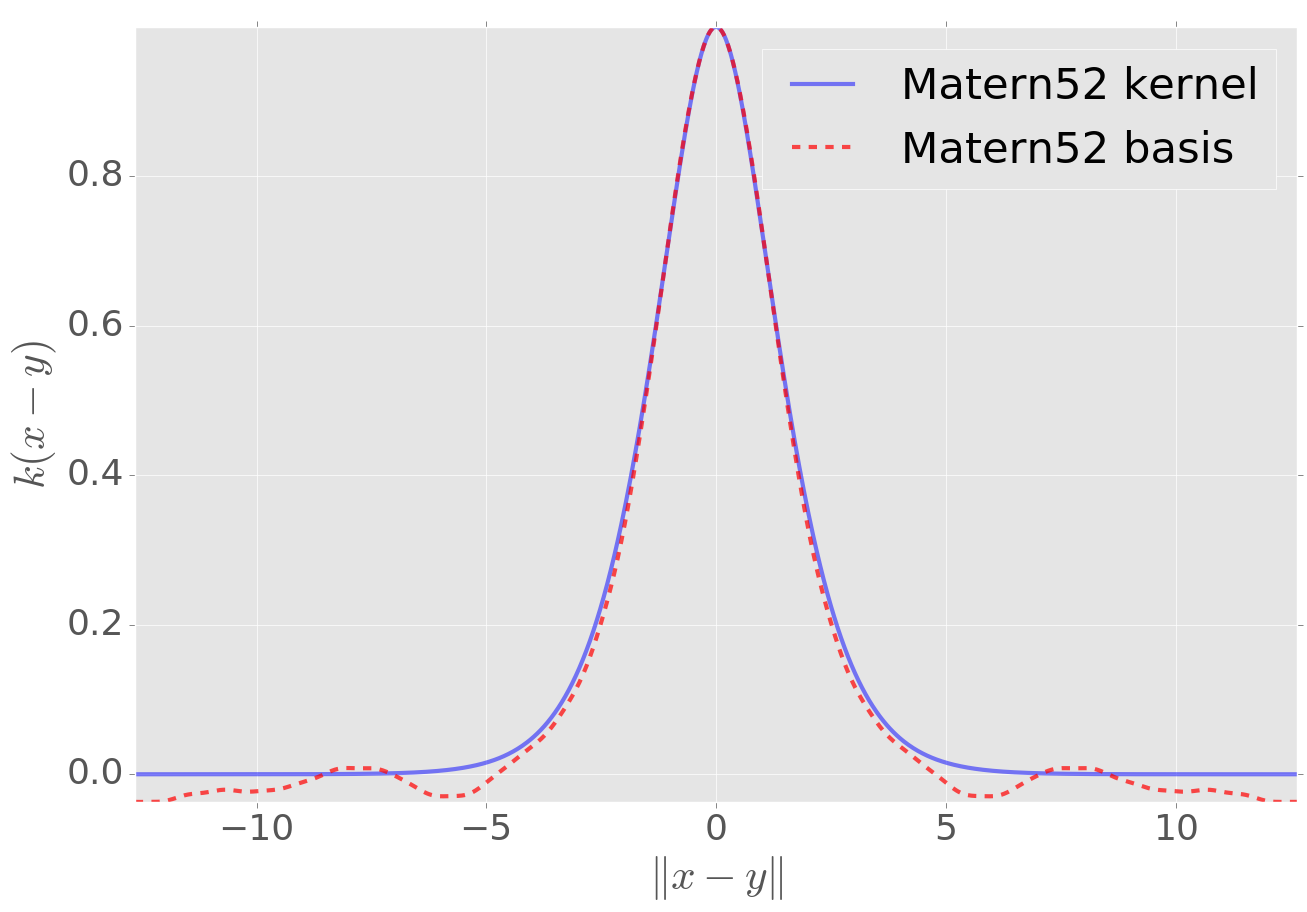
\includegraphics[width=0.47\linewidth]{figs/matern52.png}
        \label{fig:matern52}
    }\\
    \caption{Comparison of various kernels and their basis approximations. In
        each of these figures 1500 random bases have been used, and the inputs
        to the kernels are 10 dimensional, $\inss \in \real{10}$.}
    \label{fig:kerns}
\end{figure}

An important feature of \revrand{} is that we can combine these random features
(and non-random features) to build even more expressive features. In
particular, we support basis \emph{concatenation} while still allowing basis
function hyperparameter learning,
\begin{equation}
    \feat_{\text{cat}} = \sbrac{
        \func{\featsym}{\ins, \param_1}{1},
        \func{\featsym}{\ins, \param_2}{2},
        \ldots,
        \func{\featsym}{\ins, \param_P}{P}
    }.
\end{equation}
In the following manner this approximates kernel addition,
\begin{equation}
    \reg_1 \kernl_1\!\brac{\ins, \ins, \param_1} +
    \reg_2 \kernl_2\!\brac{\ins, \ins, \param_2} + \ldots +
    \reg_P \kernl_P\!\brac{\ins, \ins, \param_P} \approx
    \feat_{\text{cat}} \Reg \feat_{\text{cat}}\T,
\end{equation}
where $\Reg = \diag{\sbrac{\reg_1 \mathbf{1}, \reg_2 \mathbf{1}, \ldots, \reg_P
        \mathbf{1}}}$ and each vector of $\mathbf{1}$ is the same dimension as
the corresponding basis. That is, the regression regularizer, or weight prior
variance in Equations \eqref{eq:slm_prior} and \eqref{eq:glm_prior}, acts as a
kernel mixing/amplitude parameter.  Kernel products also have an equivalent
representation with basis functions (outer product of bases), however we have
not yet implemented this.

We also support \emph{partial application} of basis functions to certain
dimensions of the inputs, $\ins$, while also allowing concatentation, e.g,
\begin{equation}
    \func{\featsym}{\ins, \boldsymbol\param}{} = \sbrac{
        \func{\featsym}{\ins_{1:10}, \param_1}{1},
        \func{\featsym}{\ins_{5:D}, \param_2}{2},
        \ldots,
        \func{\featsym}{\ins, \param_P}{P}
    } 
\end{equation}
Where the subscript of $\ins$ denotes (arbitrary) column slices. See
\revrand{}'s documentation on how to use this features.

\section{Experiments}

\subsection{Boston Housing Regression}

\begin{table}[htb]

    \centering
    \begin{tabular}{r|c c}
        \textbf{Algorithm} & \textbf{R-square} & \textbf{MSLL} \\
        \hline
        \emph{SLM} & 0.9018 (0.0134) & -1.504 (0.1191) \\
        % \emph{GLM} & 0.8340 (0.0491) & -0.8763 (0.1242) \\
        \emph{GLM} & 0.8411 (0.0491) & -0.9209 (0.1530) \\
        GP & \textbf{0.9027 (0.0137)} & \textbf{-1.1792 (0.1581)} \\
        RF & 0.8467 (0.0709) & N/A \\ 
        SVR & 0.6295 (0.0863) & N/A \\
        \hline
    \end{tabular}

\end{table}

\subsection{Handwritten Digits Classification}

\begin{table}[htb]

    \centering
    \begin{tabular}{r|c c}
        \textbf{Algorithm} & \textbf{Log-loss} & \textbf{Error (\%)} \\
        \hline
        \emph{GLM} & 0.1138 & \textbf{2.07} \\
        Logistic & 0.1734 & 3.62 \\
        SVC & \textbf{0.1003} & 6.99 \\
        GPC &  0.1405 & 2.59 \\
        RF & 0.1368 & 2.72 \\
        \hline
    \end{tabular}

\end{table}

\subsection{SARCOS Regression}

1 million iterations

\begin{table}[htb]

    \centering
    \begin{tabular}{r|c|c c}
        \textbf{Algorithm} & \textbf{Approximation size} & \textbf{SMSE} &
        \textbf{MSLL} \\
        \hline
        \emph{GLM} & 256 & 0.0358 & -1.6644 \\
        & 512 & 0.0252 & -1.8397 \\
        & 1024 & 0.0207 & -1.9341 \\
        & 2048 & 0.0171 & -2.0243 \\
        & 8192 & 0.0152 & -1.9804 \\
        \hline
    \end{tabular}

\end{table}

\bibliography{report}

\end{document}
